%%
%% Bioinformatics Original Paper (OUP authoring template)
%% Retargeted from Knowledge-Based Systems / Cell Press drafts
%%
\documentclass[numsec,webpdf,modern,large]{oup-authoring-template}

\pdfminorversion=5
\usepackage{booktabs}
\usepackage{amsmath}
\usepackage{amssymb}
\usepackage{xcolor}
\usepackage{xurl}
\usepackage{graphicx}

\graphicspath{{figs/}}
\newcommand{\societylogo}{}

\theoremstyle{thmstyleone}
\newtheorem{theorem}{Theorem}
\newtheorem{proposition}[theorem]{Proposition}
\theoremstyle{thmstylethree}
\newtheorem{definition}{Definition}

\newcommand{\splitname}[1]{\textit{#1}}
\newcommand{\modpath}[1]{\textit{#1}}

\begin{document}

\journaltitle{Bioinformatics}
\DOI{DOI HERE}
\copyrightyear{2026}
\pubyear{2026}
\vol{00}
\issue{0}
\access{}
\appnotes{Original Paper}

\firstpage{1}

\title[GERM-BO for genomic foundation models]{GERM-BO: a reproducible border-aware adapter framework for genomic foundation models}

\author[1]{Mingxuan Huang\ORCID{0009-0005-3428-2119}}
\author[2]{Jingchao Wang\ORCID{0000-0002-0099-539X}}
\author[1]{Miyang Yang\ORCID{0009-0006-7347-8920}}
\author[3]{Zhaochu Wang\ORCID{0009-0003-9091-6476}}
\author[4]{Dayou Chen}
\author[1,$\ast$]{Xi Sun}

\address[1]{\orgdiv{Zhongshan School of Medicine}, \orgname{Sun Yat-sen University}, \orgaddress{\street{No.\ 74 Zhongshan Road 2}, \postcode{510080}, \state{Guangzhou}, \country{China}}}
\address[2]{\orgdiv{School of Computer Science}, \orgname{Peking University}, \orgaddress{\street{No.\ 5 Yiheyuan Road, Haidian District}, \postcode{100871}, \state{Beijing}, \country{China}}}
\address[3]{\orgdiv{Department of Anorectal Surgery}, \orgname{The Affiliated People's Hospital of Fujian University of Traditional Chinese Medicine}, \orgaddress{\street{No.\ 602 Middle 817 Road}, \postcode{350004}, \state{Fuzhou}, \country{China}}}
\address[4]{\orgdiv{School of Computer Science}, \orgname{Sun Yat-sen University}, \orgaddress{\street{No.\ 132 Waihuan East Road, Guangzhou University City}, \postcode{510006}, \state{Guangzhou}, \country{China}}}

\corresp[$\ast$]{Corresponding author. \href{mailto:sunxi2@mail.sysu.edu.cn}{sunxi2@mail.sysu.edu.cn}}

\abstract{%
\textbf{Motivation:}
Resource-efficient adaptation of genomic foundation models often relies on outlier suppression and low-rank adapters, but uniform suppression can attenuate bursty, self-overlapping DNA-token directions that carry task signal.\\
\textbf{Results:}
We present GERM-BO, a LoRA-compatible compensation channel driven by overlap-based border scores. Under oracle metadata scores, GERM-BO improves DNABERT-2 accuracy by $+0.114$ on a controlled hard-border split. On a strict 3-mer-balanced splice benchmark with label-free scores, quantile-normalized GERM-BO improves macro-F1 by $+0.091$ over the matched LoRA baseline and recovers non-dominant splice classes. Ablations show that the gain requires correctly aligned compensation rather than generic gating.\\
\textbf{Availability and Implementation:}
Source code, processed splits, YAML configs, and reproduction scripts are freely available under the MIT license at \url{https://github.com/hhhhmx/GERM-BO} (Python/PyTorch; single-GPU). The archived release with DOI is \url{https://doi.org/10.5281/zenodo.PENDING} (replace after Zenodo minting; see repository \texttt{CREATE\_ZENODO\_DOI.md}).\\
\textbf{Contact:} \href{mailto:sunxi2@mail.sysu.edu.cn}{sunxi2@mail.sysu.edu.cn}\\
\textbf{Supplementary information:}
Supplementary data are available at \textit{Bioinformatics} online.}

\keywords{genomic foundation models, parameter-efficient fine-tuning, DNA word overlap, activation outliers, splice sites}

\maketitle

\section{Introduction}\label{sec:introduction}

Genomic foundation models transfer pretrained DNA representations to promoters, splice sites, and chromatin tasks~\cite{dnabert2021,dnabert22023,nucleotidetransformer2024,hyenadna2024,jaganathan2019spliceai}. In practice, users often rely on parameter-efficient fine-tuning (PEFT) rather than full updates. Outlier-aware adaptation and quantization improve efficiency under limited compute~\cite{germ2025,dettmers2022llm,lora2022}, but treat tokens largely as generic features.

Genomic tokens are not generic words~\cite{lindsey2025impact}. Finite-alphabet self-overlap induces short-range recurrence and burst-like activations~\cite{guibas1981string,Dai2011,bondarenko2021understanding}, so a large response can be both a computational outlier and a task-relevant motif signal~\cite{Kinney2010,zhou2015predicting}. Existing PEFT analyses do not identify which overlap-rich directions are hit hardest by uniform suppression, nor how to compensate them without raising the trainable rank (Fig.~\ref{fig:motivation}).

\begin{figure}[!t]
\centering
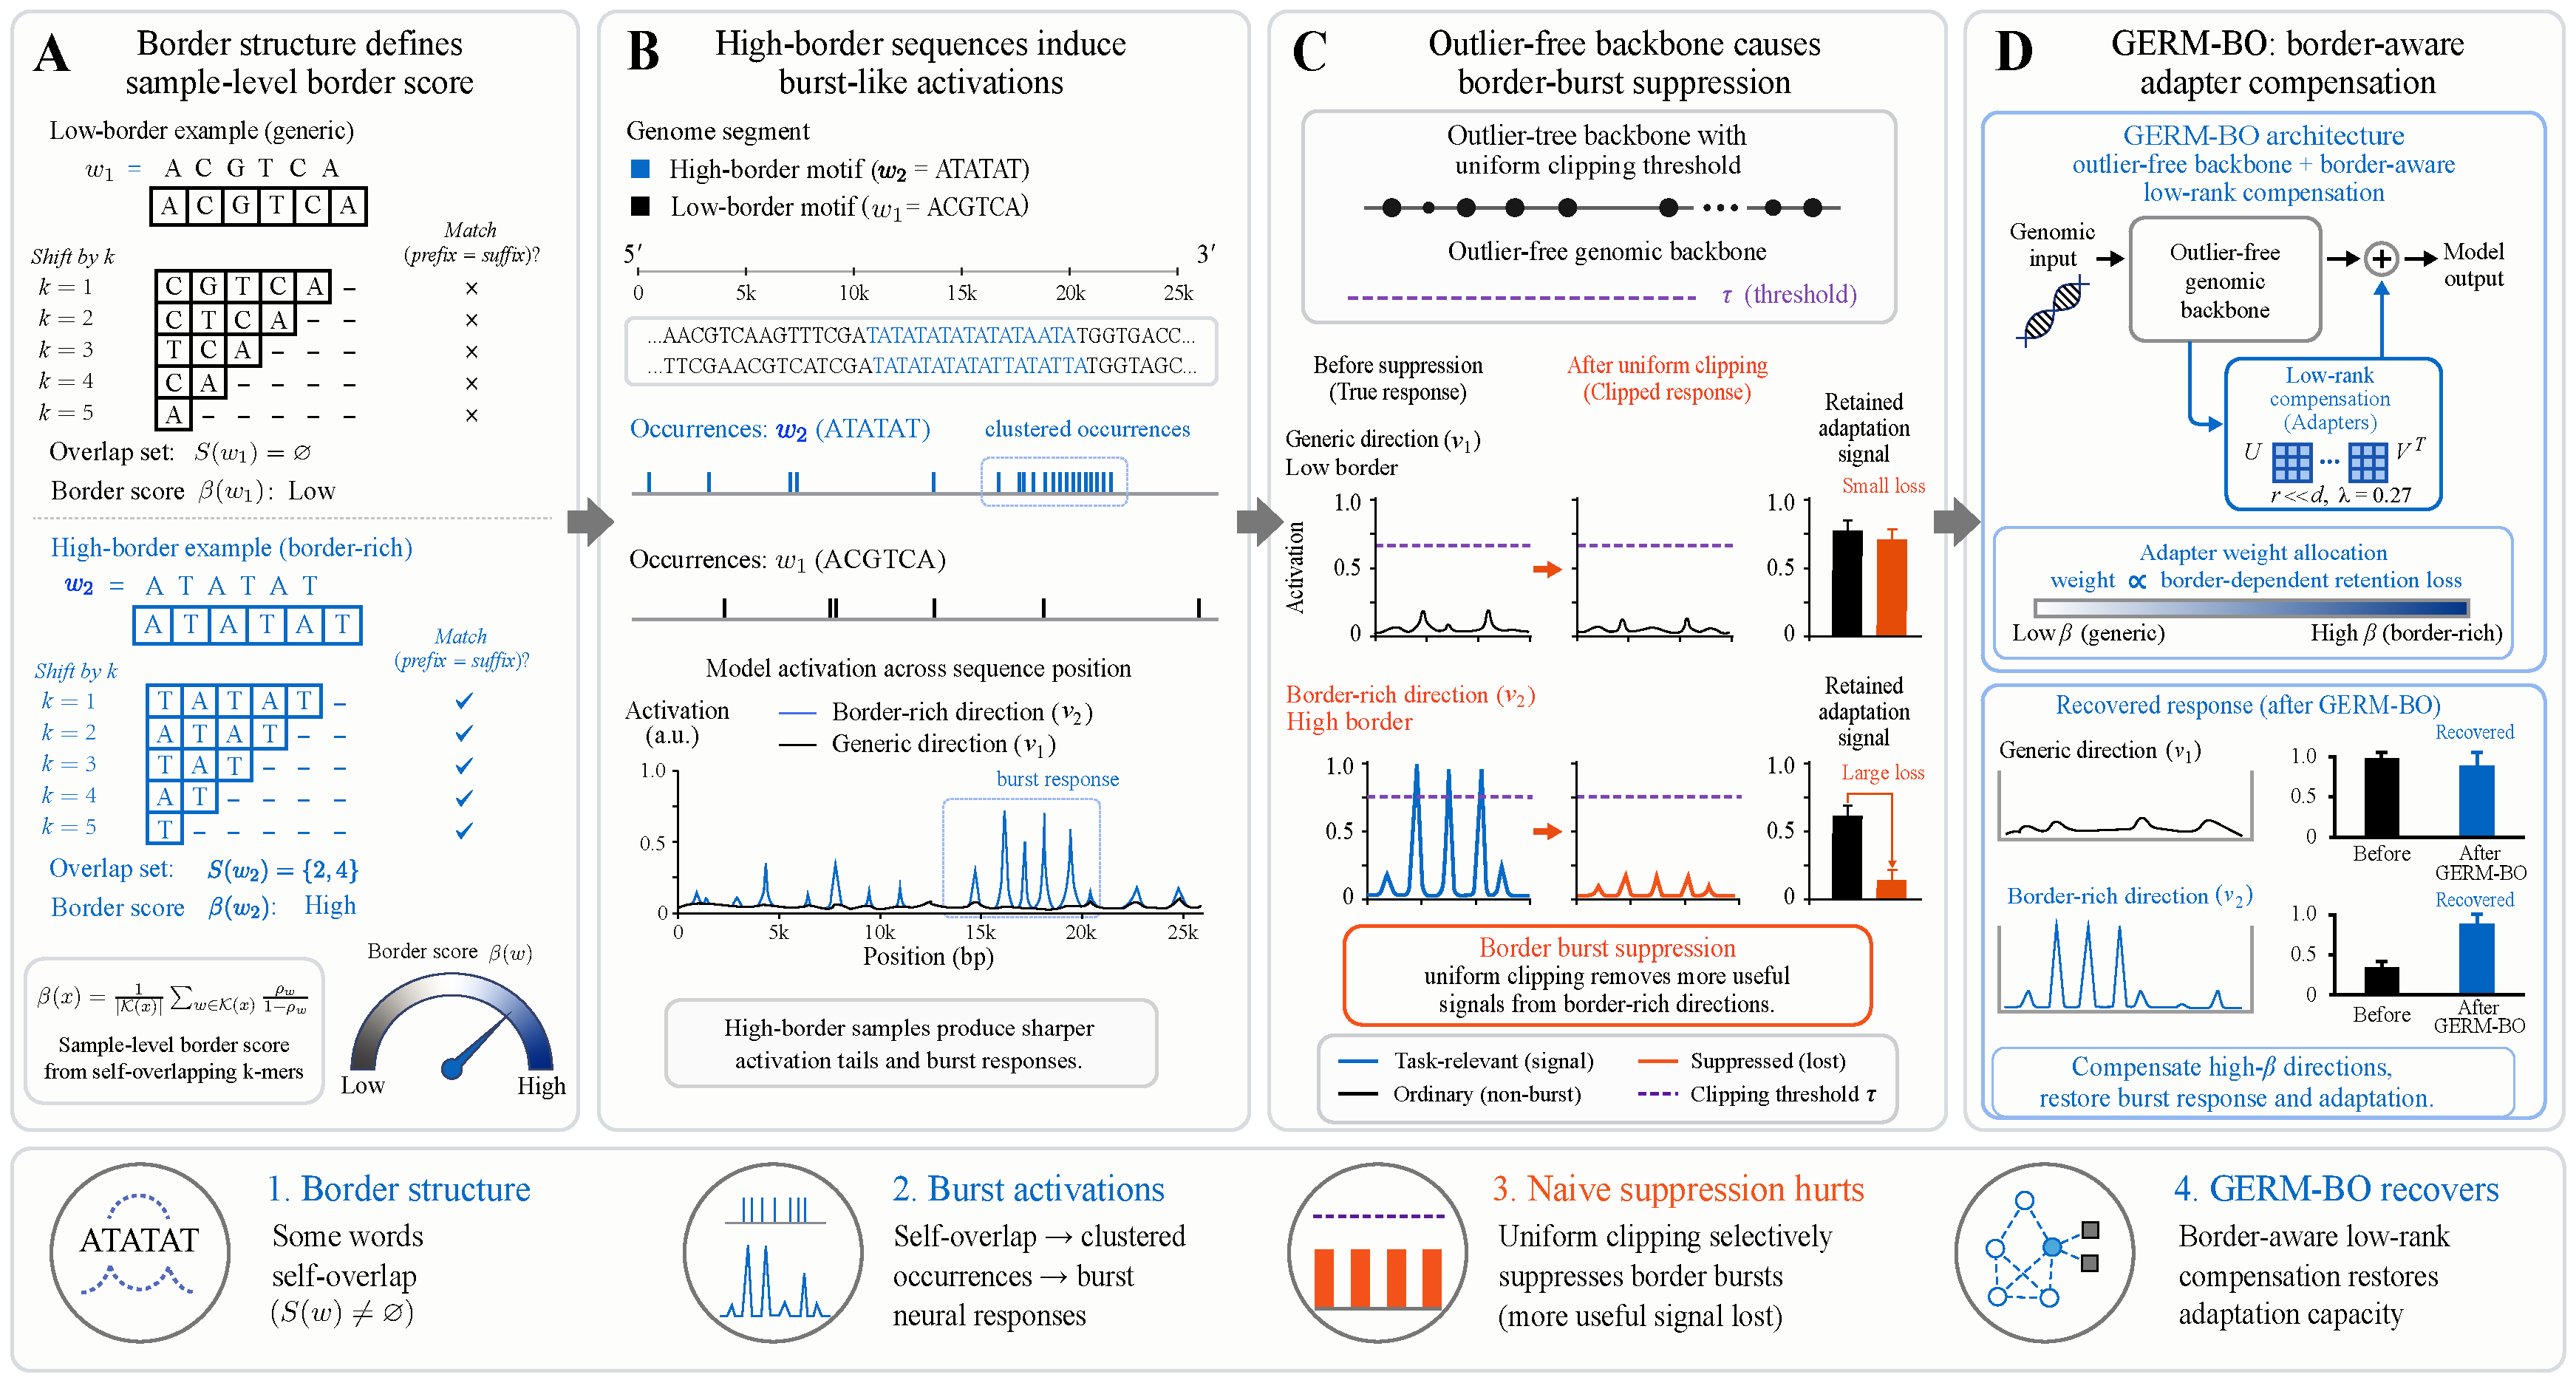
\includegraphics[width=\linewidth]{figs/fig1.pdf}
\caption{Self-overlapping genomic tokens induce clustered occurrences and burst-like activations. Uniform clipping disproportionately removes signal in high-border directions; GERM-BO restores capacity via border-aware LoRA compensation.}
\label{fig:motivation}
\end{figure}

We introduce GERM-BO, a reusable adapter framework that keeps the backbone and LoRA rank fixed while multiplying the adapter branch by a border-derived compensation factor. Contributions: (i)~overlap-based border scoring for DNA words; (ii)~border-burst suppression as the design principle for compensation (proofs in Supplementary Note~S1); (iii)~a drop-in LoRA implementation using metadata, activation-derived, or label-free scores; (iv)~controlled and strict splice protocols that separate genuine gains from short $k$-mer shortcuts, with explicit null regimes on promoters and histone marks.

Related genomic LMs~\cite{dnabert22023,nucleotidetransformer2024,hyenadna2024}, PEFT/quantization methods~\cite{adapters2021,lora2022,qlora2023,germ2025}, and word-overlap combinatorics~\cite{guibas1981string,wordstats2022} motivate the gap; GERM-BO links overlap geometry to adapter allocation under outlier suppression.

\section{System and methods}\label{sec:methods}

\subsection{Border-burst suppression}

For a word $w=w_1\cdots w_m$, the overlap set is
\begin{equation}
S(w)=\{\ell\in\{1,\ldots,m-1\}\mid w_{1:m-\ell}=w_{\ell+1:m}\}.
\label{eq:overlapset}
\end{equation}
Under a stationary Markov background, continuation mass $\rho_w=\sum_{\ell\in S(w)}q_w(\ell)$ yields the border score $\beta_w=\rho_w/(1-\rho_w)$ (assuming $\rho_w<1$). In the rare-word renewal approximation, expected local cluster length equals $1+\beta_w$ (Supplementary Note~S1).

Let $q_{\tau}$ be a clipping map with derivative $\phi_{\tau}$, and let $a_w$ and $g_w$ be activation and task-gradient responses aligned with $w$. Retained information after suppression is
\begin{align}
I_w(\tau)&=\mathbb{E}[\phi_{\tau}(a_w)^2 g_w^2],&
R_w(\tau)&=I_w(\tau)/I_w(\infty).
\label{eq:retention}
\end{align}
\begin{theorem}\label{thm:fisher}
Under the scale model $a_w\overset{d}{=}b_0(1+\beta_w)Z$ and independence assumptions in Supplementary Note~S1, if $\beta_{w_1}\le\beta_{w_2}$ then $R_{w_1}(\tau)\ge R_{w_2}(\tau)$ for every fixed $\tau>0$.
\end{theorem}
Thus the same outlier control that improves average efficiency can disproportionately reduce information in high-border directions (Fig.~\ref{fig:method}).

\begin{figure}[!t]
\centering
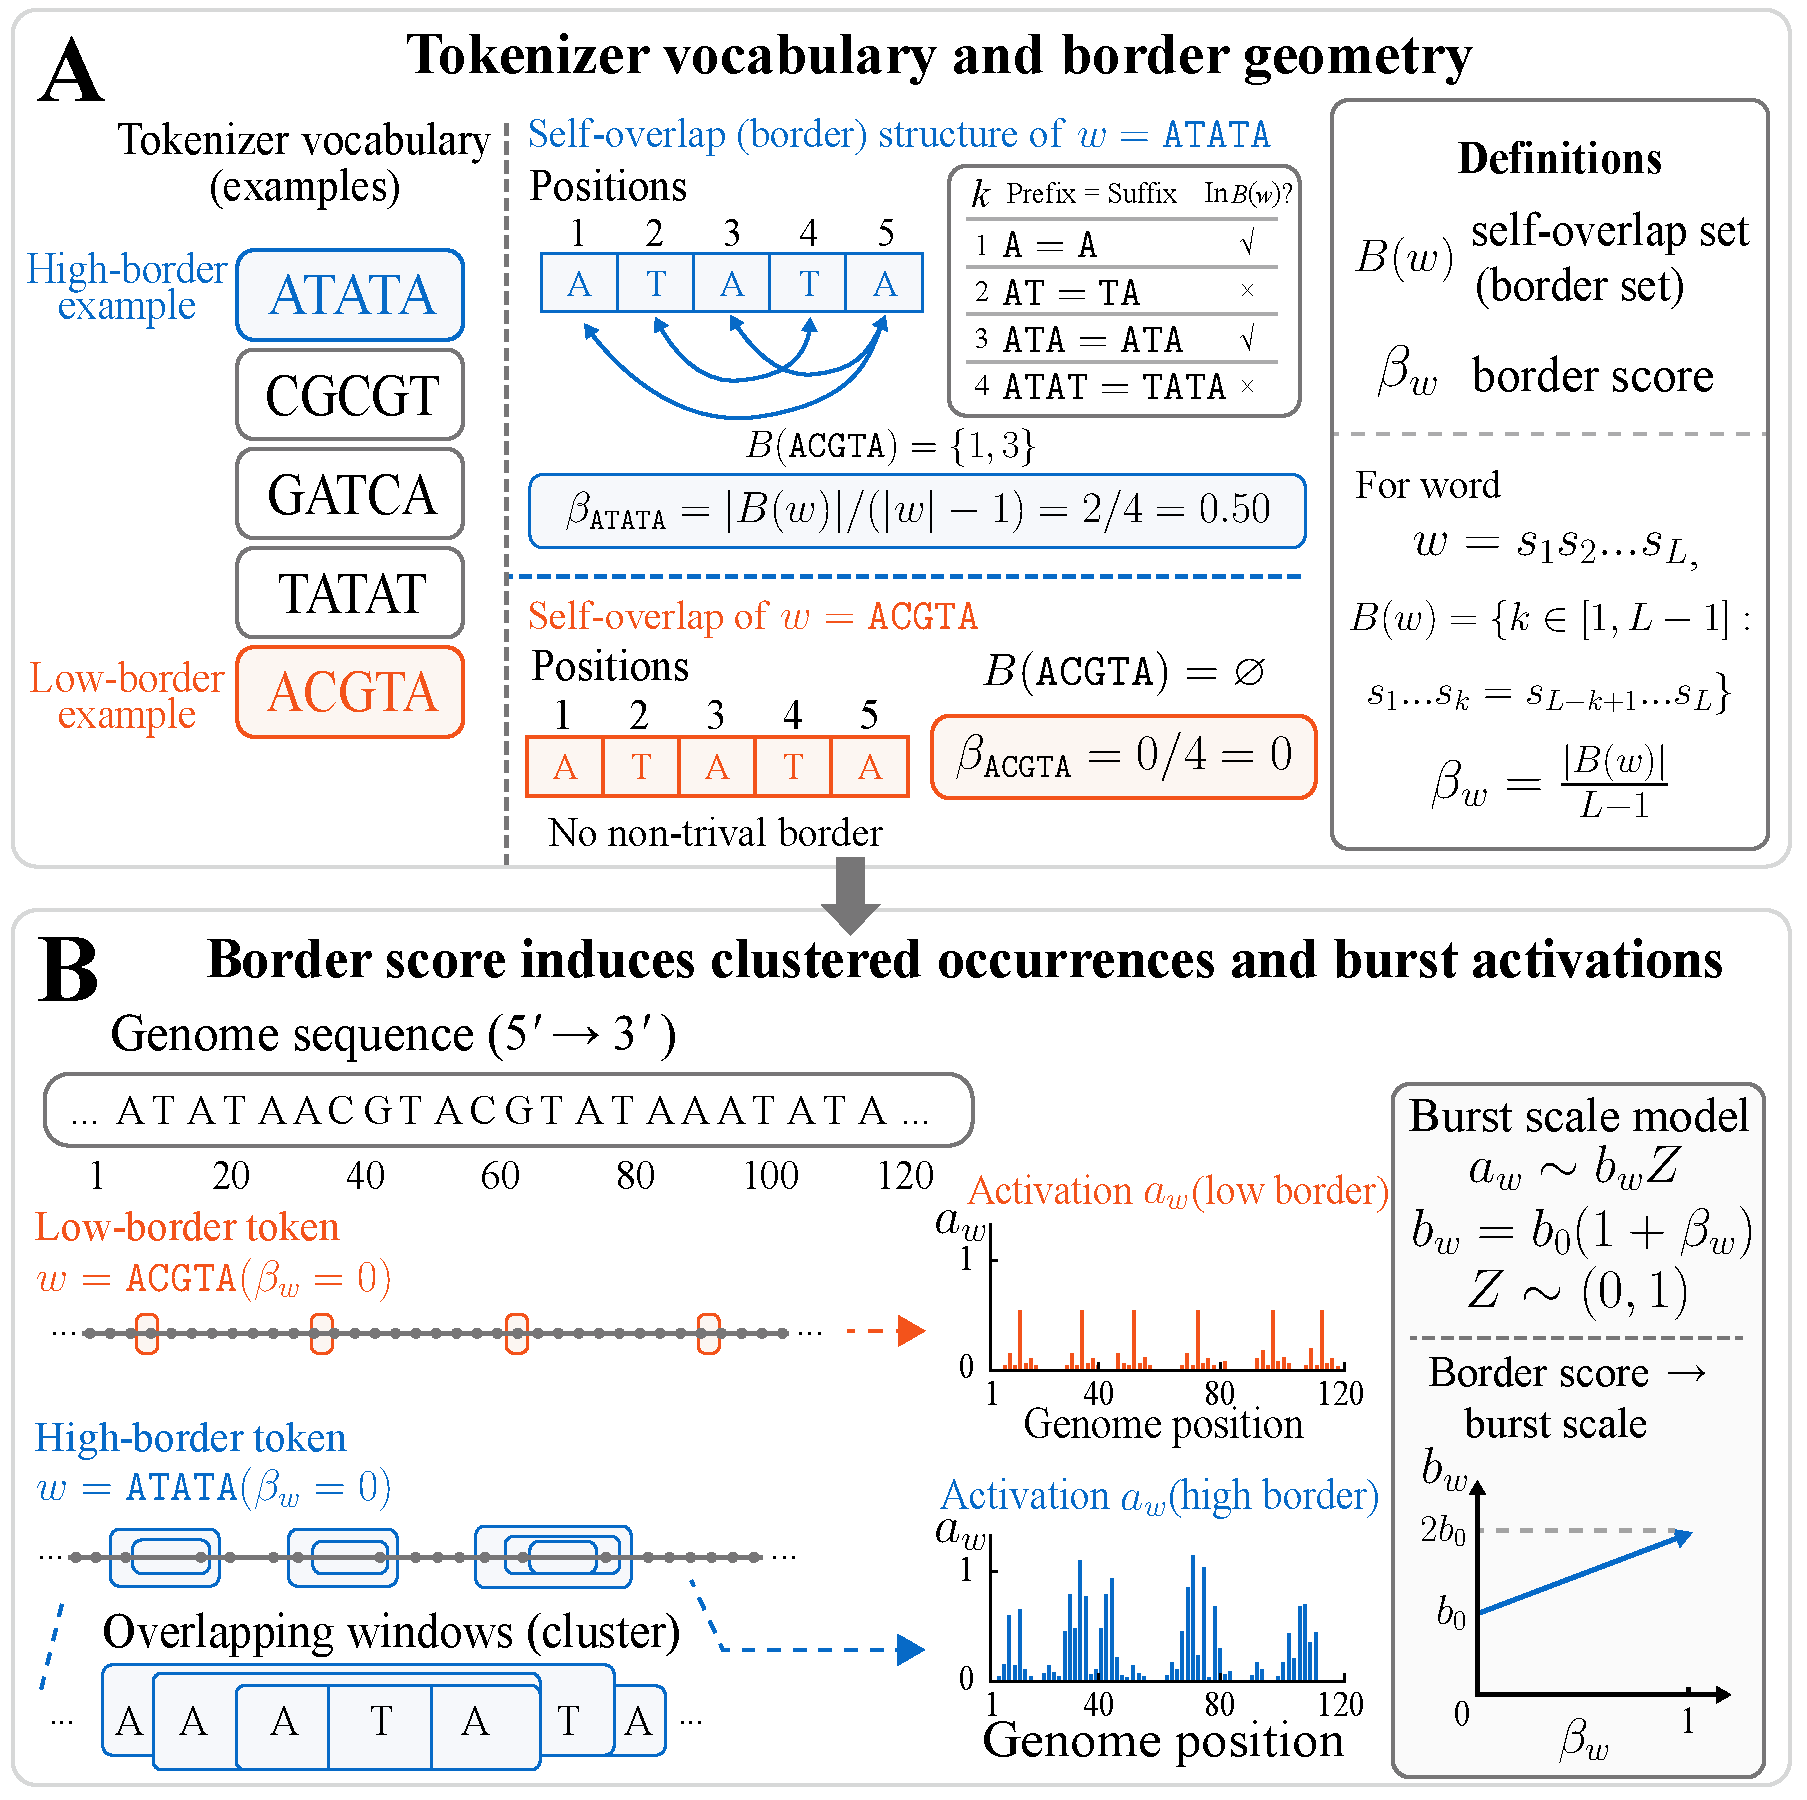
\includegraphics[width=\linewidth]{figs/fig2_ab.pdf}
\caption{Border score $\beta_w$ from token self-overlap (A) and border-burst suppression: retention $R_w(\tau)$ decreases with $\beta_w$ under uniform clipping (B).}
\label{fig:method}
\end{figure}

\subsection{GERM-BO adaptation rule}

Idealized token-aligned compensation augments LoRA $\Delta W=BA$ as $\Delta W=BA\Gamma$ with diagonal weights $\gamma_w=(1+\beta_w)^{\alpha}$. The deployed trainer instead multiplies the LoRA branch by a per-sample factor
\begin{equation}
c(x)=\mathrm{clip}\!\Bigl(1+\lambda_{\mathrm{comp}}\bigl(s(x)/\mathbb{E}_{\mathrm{batch}}[s]-1\bigr),\,c_{\min},\,c_{\max}\Bigr),
\label{eq:implcomp}
\end{equation}
where $s(x)$ is a metadata, activation-derived, or sequence-estimated border score, and the forward map is $y=Wx+\mathrm{scale}\cdot B(A(\mathrm{dropout}(x))\cdot c(x))$ (Fig.~\ref{fig:comp}). Default controlled settings use $\lambda_{\mathrm{comp}}=0.27$ with clip $[0.73,1.42]$; the strict splice protocol uses quantile-normalized scores clipped to $[0.8,1.2]$.

\begin{figure}[!t]
\centering
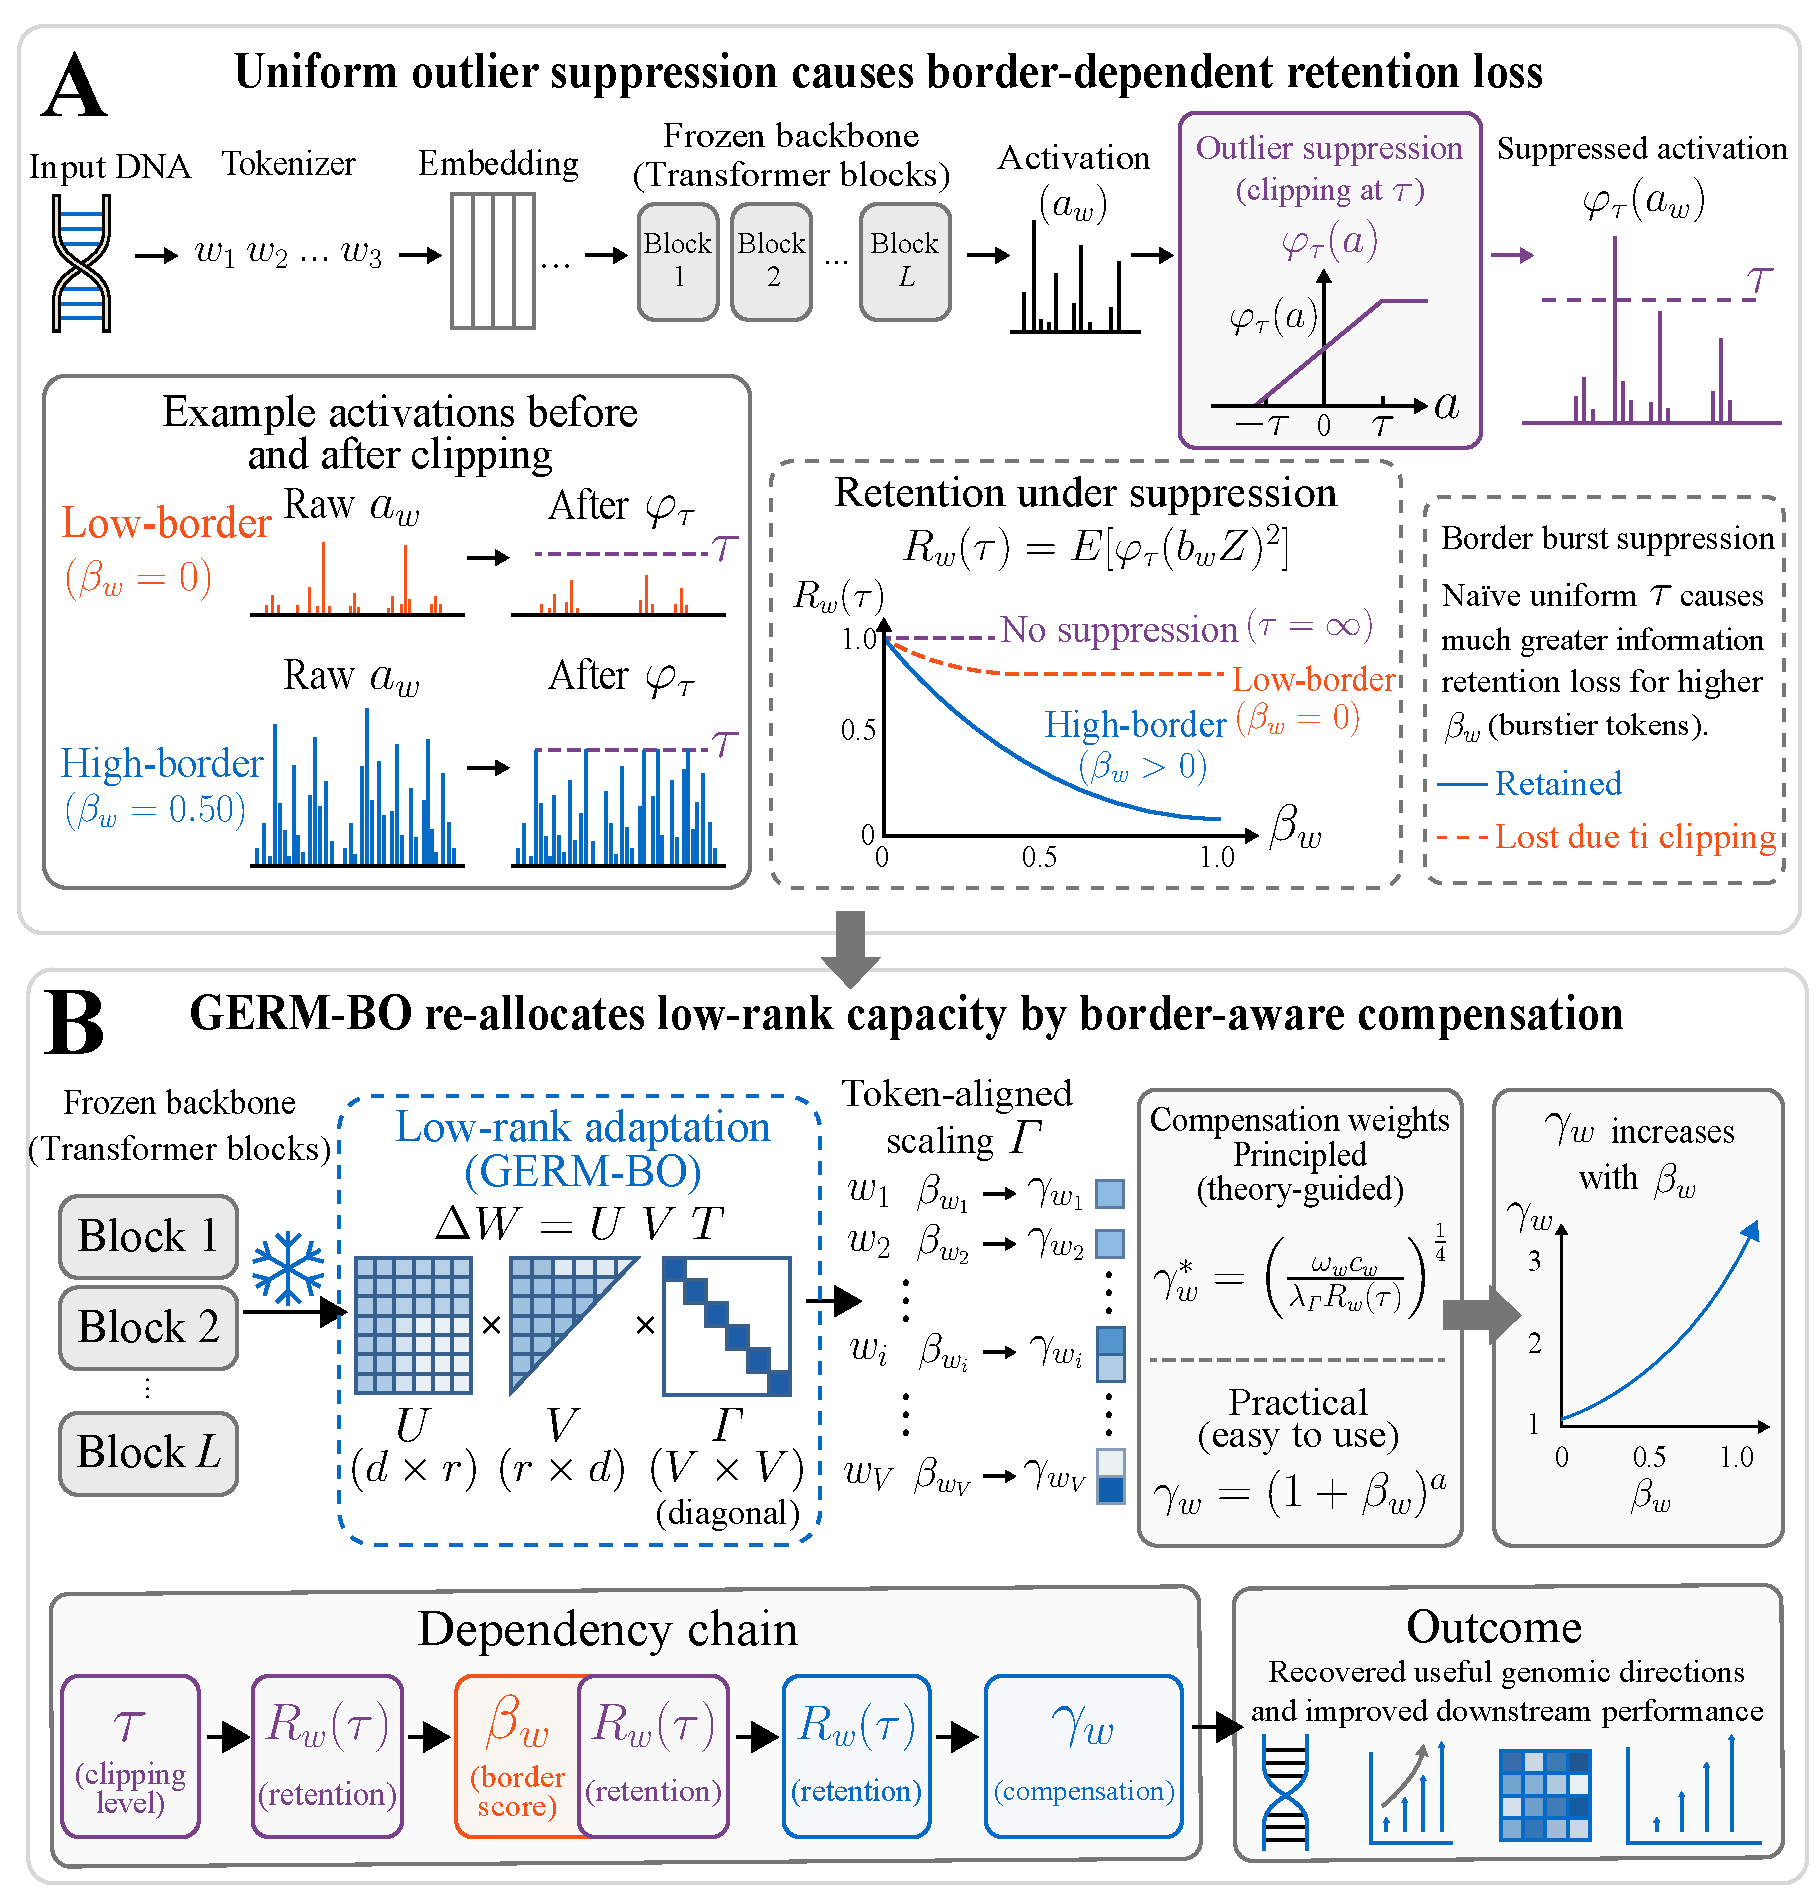
\includegraphics[width=\linewidth]{figs/fig2_cd.pdf}
\caption{GERM-BO compensation: LoRA update with diagonal $\Gamma$ in the token-aligned view (C) and capacity reallocation toward high-border directions (D).}
\label{fig:comp}
\end{figure}

\subsection{Training data and homology controls}

Unless noted, experiments use DNABERT-2 (117M) with LoRA on \modpath{attention.output + classifier}, AdamW, early stopping on validation accuracy, and single-GPU training. We never report cross-validation averages in place of an independent test set: each run selects the checkpoint by validation accuracy and then evaluates once on a held-out test split that is unused for training or model selection.

\paragraph{Controlled border-aware splits.}
Synthetic sequences are built so that sample-level border scores are known by construction. The main controlled split \splitname{hard\_border\_large} contains $1024/256/256$ train/validation/test examples; the held-out mechanism splits \splitname{border\_easy}, \splitname{border\_medium}, and \splitname{border\_hard} use the same $1024/256/256$ sizes. Because these sequences are generated rather than sampled from a natural genome, classical sequence-homology leakage between partitions is not the primary concern; the relevant control is score alignment (metadata vs.\ shuffled metadata), reported in Supplementary Table~S1.

\paragraph{Strict splice protocol (real biological data).}
External evaluation uses real splice-site windows from the Nucleotide Transformer downstream collection~\cite{nucleotidetransformer2024} (\texttt{splice\_sites\_all}; three classes: acceptor, donor, non-splice). Short $3$-mer composition induces train--test shortcuts under naive random splits, which is a homology/composition leakage mode for short DNA windows~\cite{jaganathan2019spliceai,zhang2023pangolin}. We therefore build a strict \splitname{3-mer-balanced} partition that (i)~matches examples across labels on GC bin and dominant $3$-mer signature so that class-conditional oligonucleotide neighborhoods are shared, (ii)~allocates disjoint signature keys to train, validation, and test so near-identical local contexts are not reused across partitions, and (iii)~enforces class balance. The released balanced split sizes are $9000/1800/1800$ train/validation/test with $3000/600/600$ sequences per class. Label-free border scores use center-window $k$-mer Jensen--Shannon divergence without class labels, then train-quantile normalization fitted on the training split only. Secondary promoter and histone pilots use fixed pilot (seeds 42--44) and held-out (seeds 45--49) protocols with $2000/500/1000$ subsets (Supplementary Note~S2). Metrics are test accuracy and (macro-)F1 as mean$\pm$std over seeds, with paired bootstrap intervals for key comparisons.

\section{Results}\label{sec:results}

\subsection{Controlled border-aware validation}

On \splitname{hard\_border\_large} (13 seeds; Table~\ref{tab:controlled-main}; Fig.~\ref{fig:controlled}), metadata-driven GERM-BO reaches $0.9519\pm0.0443$ accuracy versus $0.8377\pm0.0544$ for LoRA ($+0.1142$; bootstrap 95\% CI $[+0.0703,+0.1593]$; wins on $92.3\%$ of seeds). Activation-derived GERM-BO is intermediate ($0.8918\pm0.0255$). On held-out \splitname{border\_medium+hard}, metadata compensation ($0.9272\pm0.0583$) beats no compensation, activation-derived compensation, and shuffled metadata ($0.8638\pm0.0598$), confirming that aligned border scores---not a trivial side channel---drive the gain (Supplementary Table~S1). Cross-backbone oracle-metadata replication on Nucleotide Transformer v2 50M and HyenaDNA tiny likewise favors GERM-BO (Supplementary Table~S2).

\begin{table}[!t]
\centering
\caption{Controlled main result on \splitname{hard\_border\_large} (13 seeds).}
\label{tab:controlled-main}
\small
\begin{tabular}{lcc}
\toprule
Method & Accuracy & F1 \\
\midrule
Baseline LoRA & $0.8377 \pm 0.0544$ & $0.8300 \pm 0.0725$ \\
GERM-BO (Act) & $0.8918 \pm 0.0255$ & $0.8896 \pm 0.0276$ \\
GERM-BO (Meta) & $\mathbf{0.9519 \pm 0.0443}$ & $\mathbf{0.9493 \pm 0.0483}$ \\
\bottomrule
\end{tabular}
\end{table}

\begin{figure}[!t]
\centering
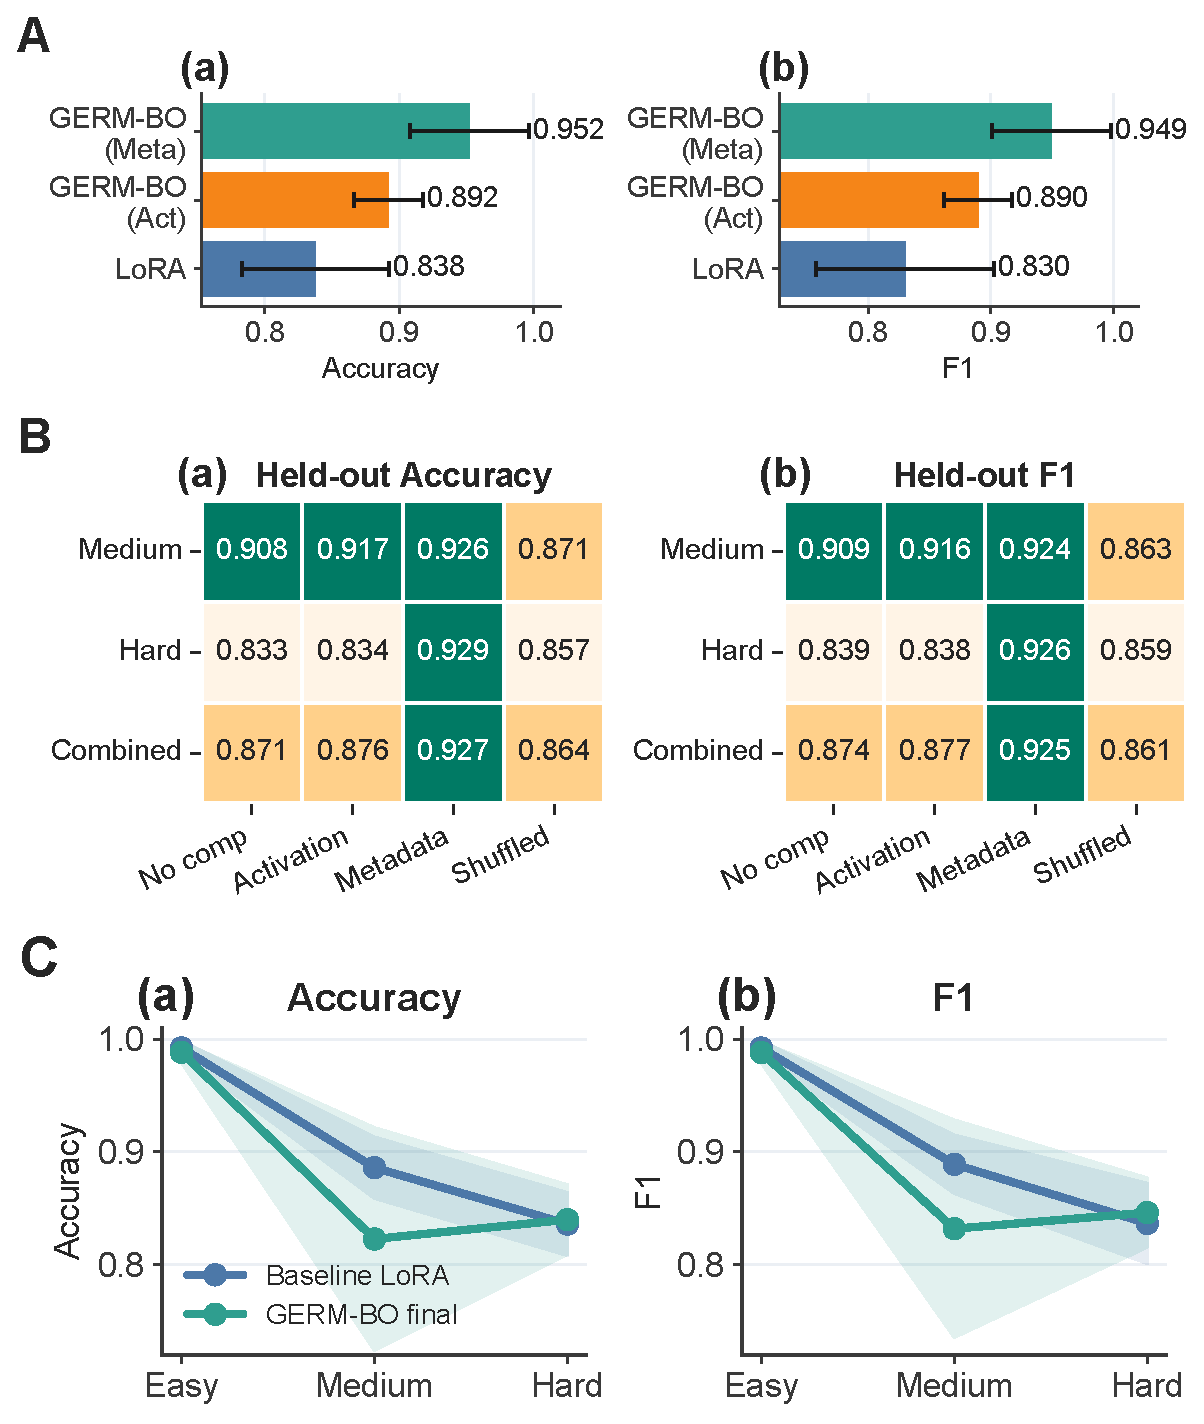
\includegraphics[width=\linewidth]{figs/010203.pdf}
\caption{Controlled results: LoRA vs.\ activation- and metadata-driven GERM-BO (A); mechanism heatmaps including shuffled metadata (B); difficulty trends (C).}
\label{fig:controlled}
\end{figure}

\subsection{Strict splice benchmark}

On the original splice split, $3$-mer linear models outperform DNABERT-2-family adapters via short-range shortcuts; the strict 3-mer-balanced split weakens this shortcut while preserving a boundary-sensitive task (Fig.~\ref{fig:splice}; Supplementary Fig.~S1). Pooled over seeds 50--59, quantile-normalized GERM-BO (Q) improves over LoRA-ATT from $0.3476\pm0.0081$ to $0.3724\pm0.0302$ accuracy ($+0.0249$; CI $[+0.0072,+0.0434]$) and from $0.2339\pm0.0282$ to $0.3245\pm0.0715$ macro-F1 ($+0.0906$; CI $[+0.0396,+0.1392]$; paired $t$-test $p=0.0008$; Table~\ref{tab:external-main}; Fig.~\ref{fig:arch}).

\begin{table}[!t]
\centering
\caption{Strict \splitname{3-mer-balanced} splice result (seeds 50--59).}
\label{tab:external-main}
\small
\begin{tabular}{lcc}
\toprule
Method & Accuracy & Macro-F1 \\
\midrule
LoRA-ATT & $0.3476 \pm 0.0081$ & $0.2339 \pm 0.0282$ \\
GERM-BO (Q) & $\mathbf{0.3724 \pm 0.0302}$ & $\mathbf{0.3245 \pm 0.0715}$ \\
\bottomrule
\end{tabular}
\end{table}

\begin{figure}[!t]
\centering
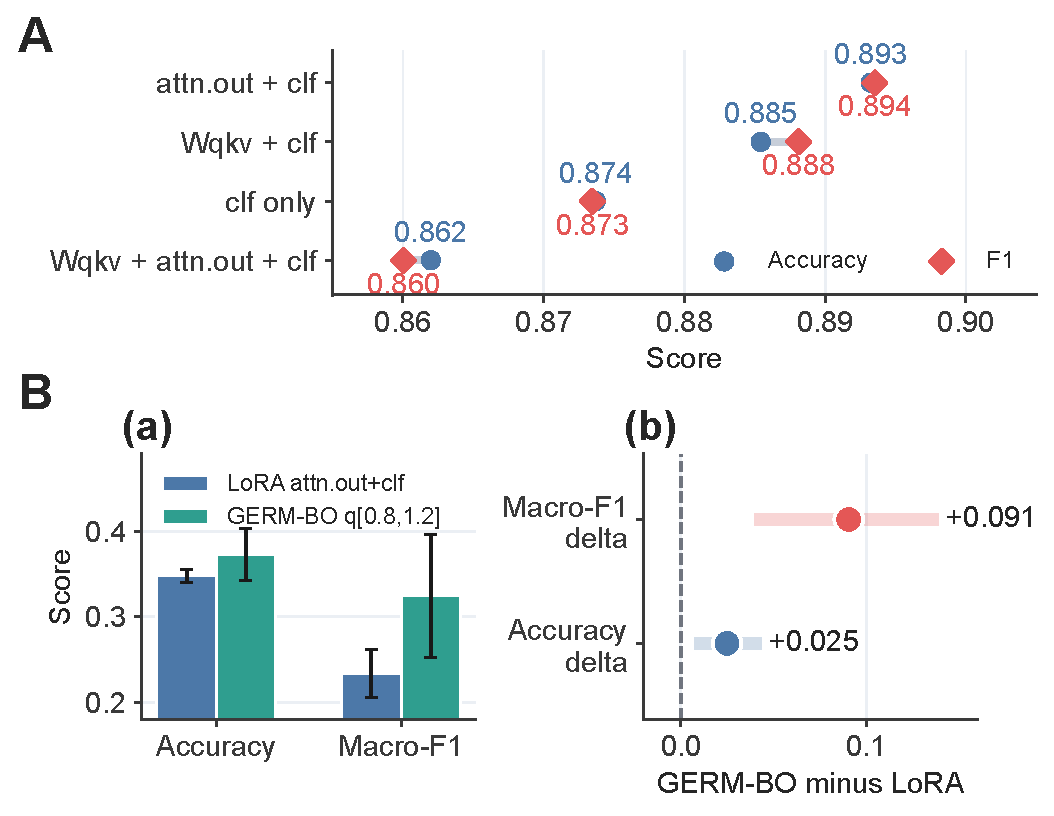
\includegraphics[width=\linewidth]{figs/0408.pdf}
\caption{Target-module ablation (A) and pooled LoRA vs.\ GERM-BO (Q) confirmation on the strict splice split (B).}
\label{fig:arch}
\end{figure}

\begin{figure}[!t]
\centering
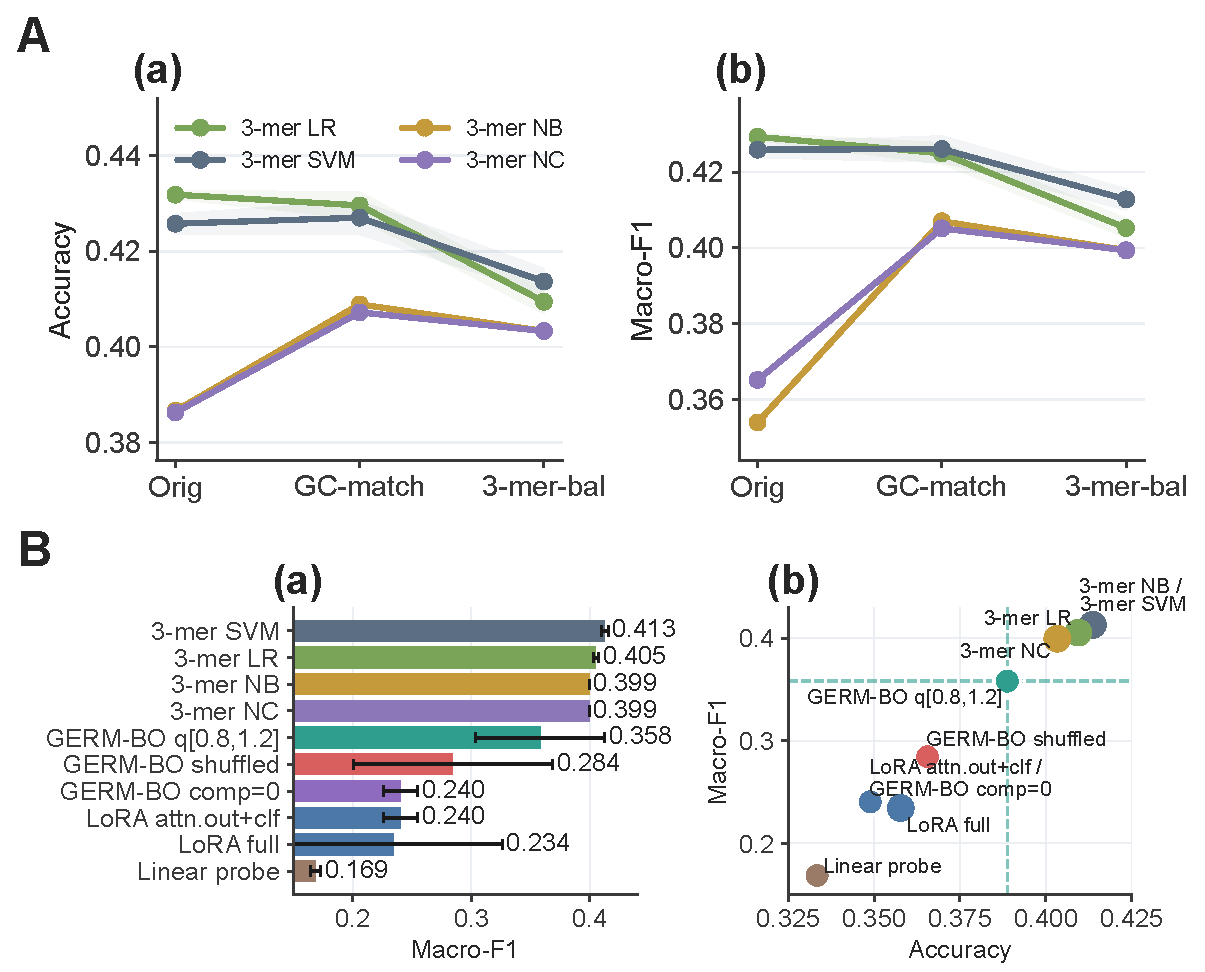
\includegraphics[width=\linewidth]{figs/0607.pdf}
\caption{Shortcut analysis across original, GC-matched, and 3-mer-balanced splits (A) and full method ranking on the strict split (B).}
\label{fig:splice}
\end{figure}

\modpath{GERM-BO comp=0} matches LoRA-ATT numerically, whereas compensated GERM-BO (Q) is substantially stronger, isolating compensation as the source of gain. On seeds 50--54, GERM-BO (Q) also outperforms input-gated LoRA and activation-derived GERM-BO on macro-F1 (Supplementary Table~S3). Per-class analysis shows recovery of acceptor/donor F1 with reduced collapse onto the dominant non-splice class (Supplementary Fig.~S2; Supplementary Table~S4). Absolute scores remain below the best $3$-mer SVM ($0.4128$ macro-F1); we claim a DNABERT-2-family improvement under a strict protocol, not universal superiority over composition baselines.

\subsection{Scope and null regimes}

Label-free GERM-BO is near-null on \splitname{human\_nontata\_promoters} ($\Delta=-0.0010$ accuracy). Histone and enhancer pilots show unstable sign across pilot vs.\ held-out seeds; label-free transfer on NT/HyenaDNA under the same splice protocol is inconclusive or near-null (Supplementary Note~S2). Thus GERM-BO helps when border structure is informative and score estimation is adequate, and we report where it currently does not.

\section{Discussion}\label{sec:discussion}

GERM-BO turns DNA-word overlap into a practical PEFT compensation channel under outlier-aware adaptation. Controlled oracle-score experiments establish the mechanism; the strict splice protocol shows a reproducible external macro-F1 gain with class recovery; shuffled-score and gated-LoRA ablations argue against generic side effects. Limitations include simplifying assumptions in Theorem~\ref{thm:fisher}, DNABERT-2-centered external gains under label-free scoring, and remaining gaps to strong $k$-mer baselines. Future work includes vocabulary-aligned token--word $\Gamma$, stronger label-free estimators, and dedicated TFBS benchmarks.

\section*{Acknowledgements}
Mingxuan Huang, Jingchao Wang, Miyang Yang, and Zhaochu Wang contributed equally. Author contributions: M.H.\ (Methodology, Software, Investigation, Visualization, Writing---original draft); J.W.\ (Conceptualization, Methodology, Writing---review \& editing); M.Y.\ (Methodology, Investigation, Writing---review \& editing); Z.W.\ (Methodology, Investigation, Writing---review \& editing); D.C.\ (Writing---review \& editing); X.S.\ (Supervision, Writing---review \& editing, Funding acquisition).

\section*{Funding}
This work was supported by the Guangzhou National Laboratory Major Project (GZNL2024A01003) to Xi Sun.

\section*{Conflict of interest}
None declared.

\section*{Data availability}
Public datasets and pretrained backbones are cited in the text. Code, processed splits, and reproduction scripts are freely available under the MIT license at \url{https://github.com/hhhhmx/GERM-BO}. The archived submission snapshot DOI is \url{https://doi.org/10.5281/zenodo.PENDING} (replace with the minted Zenodo DOI before ScholarOne upload; see \texttt{CREATE\_ZENODO\_DOI.md}).

\bibliographystyle{abbrvnat}
\bibliography{references}

\end{document}
